\documentclass[12pt]{article}
\usepackage{color}
\usepackage{cite}
\usepackage{geometry}                % See geometry.pdf to learn the layout options. There are lots.
\usepackage{pdflscape}        %single page landscape
                                %mode \begin{landscape} \end{landscape}
\geometry{letterpaper}                   % ... or a4paper or a5paper or ... 
%\usepackage[parfill]{parskip}    % Activate to begin paragraphs with an empty line rather than an indent
\usepackage{graphicx}
\usepackage{amssymb}
\usepackage{Sweave}
\newcommand{\etal}{\textit{et al.}}
\usepackage{hyperref}  %\hyperref[label_name]{''link text''}
                       %\hyperlink{label}{anchor caption}
                       %\hypertarget{label}{link caption}
\linespread{1.5}

\title{Co-occurrence Network Modeling}
\author{M.K. Lau}
%\date{}                                           % Activate to display a given date or no date

\begin{document}
\maketitle

\setcounter{tocdepth}{3}  %%activate to number sections
\tableofcontents

\section{Summary}
The method presented in Ara\' ujo et al. 2011 \cite{araujo2011} is aimed
at resolving networks of co-occurrence patterns from community
datasets. Although it is framed within a biogeographic context, it has
broader applicability to datasets with repeated samples of species
presence-absences. The method uses a probability framework where the
observed joint probabilities of species are tested against a null
model for their joint probabilities, which is the product of their
individual probabilities. The process for two species (a and b) given
the number of occurrences (n) and a total number of observations (N)
is based on calculating:

\begin{enumerate}
\item the individual probabilities: 
  \begin{itemize}
  \item $P(a) = \frac{n_a}{N}$
  \item $P(b) = \frac{n_b}{N}$
  \end{itemize}
\item the expected joint probability (i.e. the null expectation):
  \begin{itemize}
  \item $E[P(a,b)] = P(a) \cdot P(b)$
  \end{itemize}
\item the observed and expected number of co-occurrences:
  \begin{itemize}
  \item $n_{ab} = \frac{n_{ab}}{N}$
  \item $E[n_{ab}] = N \cdot E[P(a,b)]$
  \end{itemize}
\item the variance of the expected number of co-occurrences:
  \begin{itemize}
  \item If $E[n_{ab}] ~ bin(N,E[P(a,b)])$, then:
  \item $s^2 = N \cdot E[P(a,b)] \cdot (1 - E[P(a,b)])$ \cite{mccarthy2007}
  \end{itemize}
\item a confidence interval for the expected number of co-occurrences:
  \begin{itemize}
  \item $CI = E[n_{ab}] \pm 2 \cdot sqrt{s^2}$
  \item Note: this is a parametric approach, using either a $t$ or
    $\chi^2$ distribution for the statistic and relying on the central
    limit theorem
  \end{itemize}
\item And if $n_{ab}$ falls outside of $CI_{E[n_{ab}]}$, then the
  co-occurrence pattern is significant (i.e. non-zero)
\item Inference uses the Bray-Curtis dissimilarity of all pairs of species
  with significant co-occurrence patterns for network inference.
\item The network is further pruned using a percolation threshold
  procedure. Note: the justification for this is weak.
\end{enumerate}

The paper goes on to detail several statistics that can be calculated
from the empirical co-occurrence networks, including:

\begin{itemize}
\item Symmetry
\item Degree distribution
\item Strength distribution
\item Species degree
\item Species strength (in and out)
\end{itemize}


\section{Code}

\begin{Schunk}
\begin{Sinput}
> araujoNet <- function(x,method='bray',min.abundance=1){
+                                         #get the absent species names
+   y <- colnames(x)[apply(x,2,sum) >= min.abundance]
+                                         #remove low abundance species
+   x <- x[,apply(x,2,sum) >= min.abundance]
+                                         #assure presence-absence matrix
+   x[x!=0] <- 1
+                                         #warn if matrix is empty
+   if (ncol(x) <= 1){warning('Community matrix is empty',quote=FALSE)}else{}
+                                         #caluclate the Bray-Curtis dis.
+   d <- as.matrix(vegdist(t(x),method=method))
+                                         #calculate individual prob.
+   Pa <- apply(x,2,function(x) length(x[x!=0])/length(x))
+                                         #calculate null joint probability 
+   Pab <- array(NA,dim=c(length(Pa),length(Pa)))
+   rownames(Pab) <- colnames(Pab) <- names(Pa)
+   for (i in 1:nrow(Pab)){
+     for (j in 1:ncol(Pab)){
+       Pab[i,j] <- Pa[i]*Pa[j]
+     }
+   }
+                                         #Calculate confidence limits
+                                         #number of co-occurrences
+   N1 <- nrow(x) * Pab
+                                         #calculate the variance
+   V1 <- nrow(x) * Pab * (1-Pab)
+                                         #+/- 2 SD limits (~95% confidence)
+   cl.u <- N1 + 2*sqrt(V1)
+   cl.l <- N1 - 2*sqrt(V1)
+                                         #observed number of co-occurrences
+   Nab <- N1 * 0 
+   for (i in 1:nrow(Nab)){
+     for (j in 1:ncol(Nab)){
+       Nab[i,j] <- length(x[x[,i] != 0 & x[,j] != 0,i])
+     }
+   }
+                                         #prune within confidence limits
+   dp <- d * 0
+   dp[Nab > cl.u] <- d[Nab > cl.u]
+   dp[Nab < cl.l] <- d[Nab < cl.l]
+                                         #add back absent species
+   x.names <- c(colnames(x),y)
+   d <- cbind(d,array(0,dim=c(nrow(d),length(y))))
+   d <- rbind(d,array(0,dim=c(length(y),ncol(d))))
+   rownames(d) <- colnames(d) <- x.names
+   dp <- cbind(dp,array(0,dim=c(nrow(dp),length(y))))
+   dp <- rbind(dp,array(0,dim=c(length(y),ncol(dp))))
+   rownames(dp) <- colnames(dp) <- x.names
+                                         #pack for export
+   out <- list(x=x,d=d,dp=dp)
+   return(out)
+ }
> 
\end{Sinput}
\end{Schunk}

\section{Example}

\begin{Schunk}
\begin{Sinput}
> library(vegan)
> library(sna)
\end{Sinput}
\begin{Soutput}
     Tools for Social Network Analysis
Version      2.2-0 created on      2010-11-21.
copyright (c) 2005, Carter T. Butts, University of California-Irvine
Type help(package="sna") to get started.
\end{Soutput}
\begin{Sinput}
> data(dune)
> test <- araujoNet(dune)
> deg <- degree(test$dp[apply(test$dp,1,sum)!=0,apply(test$dp,2,sum)!=0]
+               ,rescale=FALSE)
> gplot(test$dp[apply(test$dp,1,sum)!=0,apply(test$dp,2,sum)!=0],
+       displaylabels=TRUE,gmode='graph',label.cex=0.65,
+       vertex.sides=50,vertex.col='black',edge.col='darkgrey',
+       vertex.cex=deg,edge.lwd=(test$dp[apply(test$dp,1,sum)!=0,
+                                               apply(test$dp,2,sum)!=0]+1)^2)
> 
\end{Sinput}
\end{Schunk}

The output from this function is currently a list of three
matrices. The first (x) is the presence-absence matrix used to generate
the co-occurrence network. The second (d) is the full Bray-Curtis
dissimilarity matrix. The third (dp) is the Bray-Curtis dissimilarity
matrix with the non-significant dissimilarities equal to zero. This
last matrix can easily be plotted using the \textit{gplot} function in
the \texttt{sna} package \cite{sna} (Fig. ~\ref{fig:one}).


\begin{figure} 
\begin{center} 
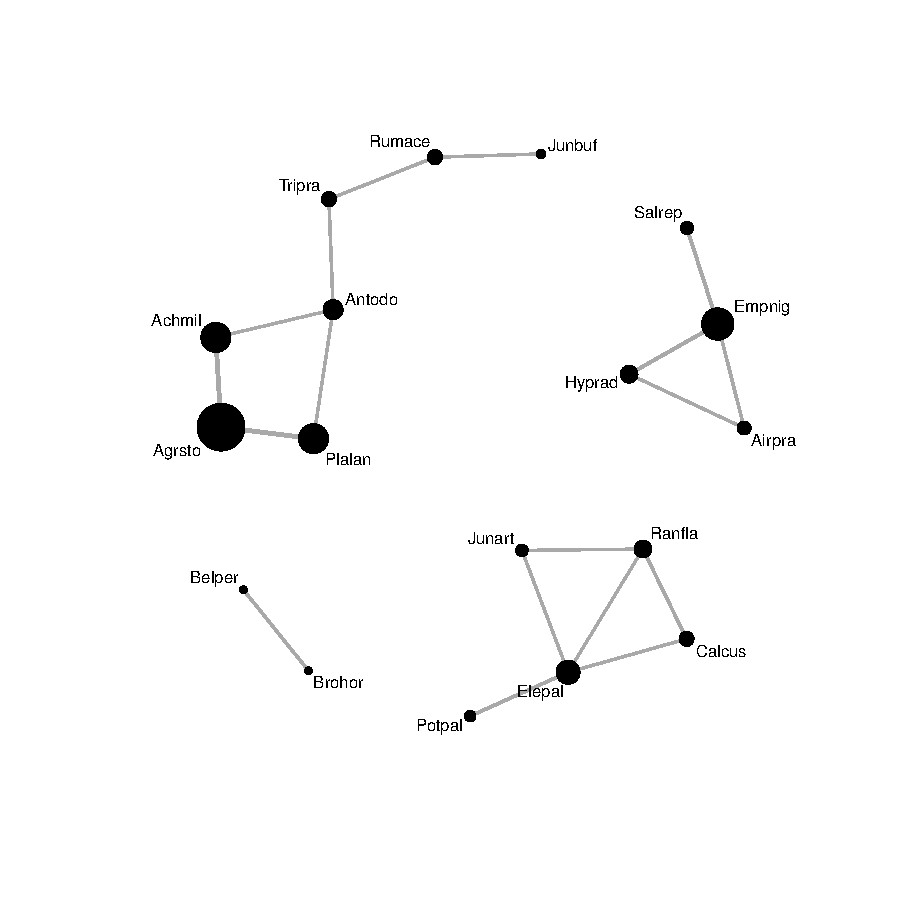
\includegraphics{araujo_method-fig1}
\end{center} 
\caption{Co-occurrence network for the \textit{dune} plant dataset in
  the \texttt{vegan} package \cite{vegan}. Species that have no significant
  co-occurrence patterns are not shown. Lines are the Bray-Curtis
  dissimilarities for pairs of species with significant joint
  probabilities. Species nodes and edges are scaled by their degrees
  and squared dissimilarities, respectively. Network figure generated
  using the \textit{gplot} function in the \texttt{sna} package
  \cite{sna}.}
\label{fig:one}
\end{figure}

%% \pagebreak
%% \section{Bayesian Co-occurrence Network}

%% <<>>=
%% library(rjags)

%% bcJP <- function(x,y,file='',nits=100,n.adapt=10,n.chains=2,diagnostics=FALSE){
%%                                         #repack data
%%   x <- cbind(x,y)
%%                                         #calculate co-occurrence
%%                                         #and number of observations
%%   x <- apply(x,1,sum)
%%   x[x!=2] <- 0
%%   x[x==2] <- 1
%%   n <- length(x)
%%   x <- sum(x)
%%                                         #create data file
%%   if (file == ''){file = 'bcn'}else{}
%%   write.table(x,file = paste(file,'.data',sep=''),row.names = FALSE,col.names = FALSE)
%%                                         #create model
%%   write.table('model{',file=paste(file,'.bug',sep=''),quote=FALSE,row.names=FALSE,col.names=FALSE)
%%   write.table('     x~dbin(p,n)',file=paste(file,'.bug',sep=''),quote=FALSE,row.names=FALSE,col.names=FALSE,append=TRUE)
%%   write.table('     p~dunif(0,1)',file=paste(file,'.bug',sep=''),quote=FALSE,row.names=FALSE,col.names=FALSE,append=TRUE)
%%   write.table('}',file=paste(file,'.bug',sep=''),quote=FALSE,row.names=FALSE,col.names=FALSE,append=TRUE)
%%                                         #initialize model
  
%%   jags <- jags.model('bcn.bug',data = list('x' = x,'n' = n),n.chains = n.chains,n.adapt = n.adapt,quiet=TRUE)
%%                                         #update model
%%   update(jags, nits,quite=TRUE)
%%                                         #sample from posterior
%%   samples <- coda.samples(jags,c('p'),nits,quiet=TRUE)
%%   if (diagnostics==TRUE){plot(samples)}else{}
%%                                         #pack for export
%%   return(c(summary(samples)$statistics[1],summary(samples)$quantiles[c(1,5)]))
%% }


%% bcNet <- function(x,method='bray',min.abundance=3){
%%                                         #get the absent species names
%%   y <- colnames(x)[apply(x,2,sum) >= min.abundance]
%%                                         #remove low abundance species
%%   x <- x[,apply(x,2,sum) >= min.abundance]
%%                                         #assure presence-absence matrix
%%   x[x!=0] <- 1
%%                                         #warn if matrix is empty
%%   if (ncol(x) <= 1){warning('Community matrix is empty',quote=FALSE)}else{}
%%                                         #caluclate the Bray-Curtis dis.
%%   d <- as.matrix(vegdist(t(x),method=method))
%%                                         #calculate individual prob.
%%   Pa <- apply(x,2,function(x) length(x[x!=0])/length(x))
%%                                         #calculate null joint probability 
%%   Pab <- array(NA,dim=c(length(Pa),length(Pa)))
%%   rownames(Pab) <- colnames(Pab) <- names(Pa)
%%   for (i in 1:nrow(Pab)){
%%     for (j in 1:ncol(Pab)){
%%       Pab[i,j] <- Pa[i]*Pa[j]
%%     }
%%   }
%%                                         #Calculate confidence limits
%%                                         #95% Posterior Credible Interval
%%   ci.l <- Pab * 0
%%   ci.u <- Pab * 0
%%   postMu <- Pab * 0
%%   count <- 0
%%   for (i in 1:ncol(x)){
%%     for (j in 1:ncol(x)){
%%       count <- count + 1
%%       if (i >= j){
%%         postJP <- bcJP(x[,i],x[,j])
%%         ci.l[i,j] <- postJP[2]
%%         ci.u[i,j] <- postJP[3]
%%         postMu[i,j] <- postJP[1]
%%         print(paste(round((count/(ncol(x)^2)*100),0),'% complete',sep=''),quote=FALSE)
%%       }else{}
%%     }
%%   }
%%                                         #fill upper matrix (matrices are summetric)
%%   ci.l[upper.tri(ci.l)] <- ci.l[lower.tri(ci.l)]
%%   ci.u[upper.tri(ci.u)] <- ci.u[lower.tri(ci.u)]
%%   postMu[upper.tri(postMu)] <- postMu[lower.tri(postMu)]
%%                                         #prune within confidence limits
%%                                         #distances/dissimilarities
%%   dp <- d * 0
%%   dp[Pab > ci.u] <- d[Pab > ci.u]
%%   dp[Pab < ci.l] <- d[Pab < ci.l]
%%                                         #posterior joint probabilities
%%   postMup <- postMu * 0
%%   postMup[Pab > ci.u] <- postMu[Pab > ci.u]
%%   postMup[Pab < ci.l] <- postMu[Pab < ci.l]
%%                                         #pack for export
%%   out <- list(x=x,d=d,dp=dp,postJP=postMu,postJPp=postMup)
%%   return(out)
%% }



%% @ 

\pagebreak
%%Activate for bibtex vibliography
\bibliographystyle{plain}
\bibliography{/Users/Aeolus/Documents/bibtex/biblib}

\end{document}  


